\documentclass{article}
\usepackage{fontspec}
\setmainfont{Libertinus Serif}
\usepackage[margin=1in]{geometry}
% Add labels to arrows
\usepackage{tikz}
%\usetikzlibrary{graphs}
%\usetikzlibrary{quotes}
\usetikzlibrary{arrows.meta}

\def\Fernandez{Fernández}
\def\Padilla{Gutiérrez de Padilla}
\def\Garcia{García de Céspedes}
\def\Vidales{Vidales}
\def\Vasquez{Vásquez}
\def\Santiago{Santiago}
\def\Lobo{Lobo}
\def\Dupont{Dupont}
\def\Jalon{Jalón}
\def\Puebla{Puebla Cathedral}
\def\Sevilla{Seville Cathedral}
\def\Malaga{Málaga Cathedral}
\def\Madrid{Madrid Royal Chapel}

\newcommand{\student}[2]{\draw[->] (#1) -- (#2)}
\newcommand{\successor}[2]{\draw[-LaTeX] (#1) -- (#2)}
\newcommand{\homage}[2]{\draw[dashed, <-] (#1)[left=10mm] -- (#2)}

\begin{document}
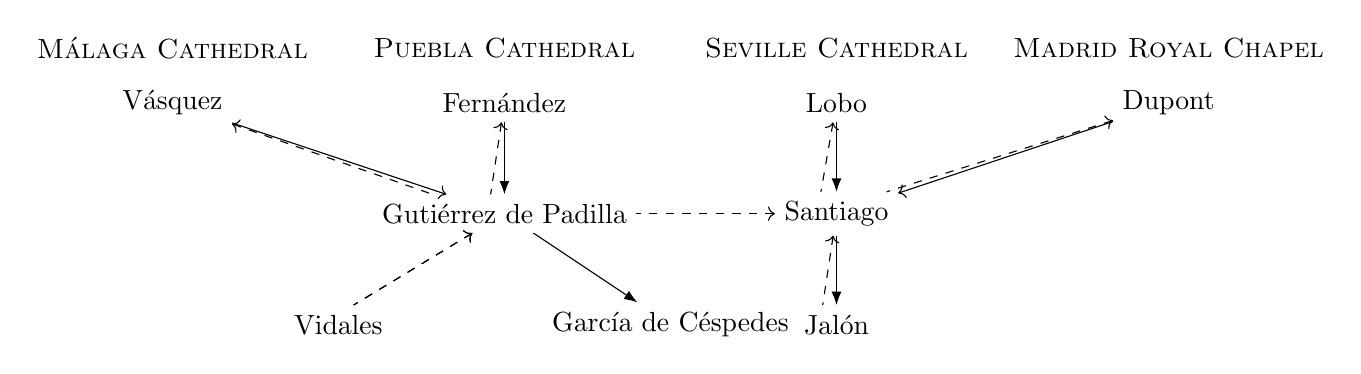
\begin{tikzpicture}[level distance=4em,
                    sibling distance=12em,
                    level 1/.style={
                        level distance=0pt,
                        font=\scshape, 
                        edge from parent/.style={draw=none}
                    },
                    level 2/.style={
                        level distance=2em,
                        font=\mdseries,
                        edge from parent/.style={draw=none}
                    },
                    level 3/.style={
                        level distance=4em,
                    }]
    \node (root) {}
        child { node (m0) {\Malaga} 
            child { node (m1) {\Vasquez} }
        }
        child { node (p0) {\Puebla}
            child { node (p1) {\Fernandez} 
                child { node (p2) {\Padilla} 
                    child { node (p3a) {\Vidales} }
                    child { node (p3b) {\Garcia} }
                }
            }
        }
        child { node (s0) {\Sevilla}
            child { node (s1) {\Lobo}
                child { node (s2) {\Santiago}
                    child { node (s3) {\Jalon} }
                }
            }
        }
        child { node (rc0) {\Madrid}
            child { node (rc1) {\Dupont} }
            };

    \student{m1}{p2};
    \homage{m1}{p2};

    \successor{p1}{p2};
    \homage{p1}{p2};

    \homage{p2}{p3a};

    \successor{p2}{p3b};
    \homage{p2}{p3a};

    \successor{s1}{s2};
    \homage{s1}{s2};
    \successor{s2}{s3};
    \homage{s2}{s3};
    \student{rc1}{s2};
    \homage{rc1}{s2};
    
    \homage{s2}{p2};
\end{tikzpicture}
\end{document}

